\documentclass{article}
\usepackage{graphicx} % Required for inserting images
\usepackage{indentfirst}
\graphicspath{ {./images/} }

\title{CTA200 Final Project Report}
\author{Joseph Tang}
\date{May 2023}

\begin{document}

\maketitle

\setlength\parindent{24pt}     
The purpose of this project was to extend Ioana Zelko's temperature map of the interstellar medium by plotting stars given in the Gaia DR3 database onto these maps. Her code loaded and plotted the temperature of the interstellar medium in 'n' bins at different distance intervals. Each distance bin was then plotted using the 'hp.mollview' function in the HEALPy library. In order to plot these stars onto the temperature map, the attached Jupyter notebook does the following.\par

Firstly, since the temperature maps do not have data for declination's less than -30°, the first function reads the Gaia csv file and deletes any lines that have declination values less than -30°. Additionally, the first function also looks for any NaN values that occur in the parallax column. Since the stars need to be separated into distance bins, any stars without parallax values would only add confusion to the maps. \par

The second function takes every parallax value and converts them into a distance value in kpc. To calculate distance from parallax, the following equation is used. 
\begin{center}
    $d (kpc) = \frac{1}{\pi (arcseconds)}$
\end{center}
Since the given parallax values are in units of milli-arcseconds, and the distance values had to be in kilo-parsecs, the equation had to be divided by $10^{6}$. These distance values were then added to the panda's dataframe. \par

The last function uses the 'SkyCoord' function in astropy.coordinates to convert from equatorial right ascension and declination values to galactic latitude and longitude. Since the temperature maps work best at galactic latitude between -60° and 60°, the code also deleted any rows that lie outside this range from the dataframe. \par

To plot the stars onto the temperature maps which were erected with hp.mollview, the dataframe searched for stars within each distance bin, took their array positions, and overlayed their latitude and longitude onto the each temperature map with hp.visufunc.projscatter. \par

The stars chosen to be plotted were type OB stars in a box of size $115 < RA < 170$, and $25 < Dec < 110$ near the Orion star forming nebula. These hot stars were chosen for their high temperatures and could provide quick correlations between type O stars and their positions relative to the temperature of the interstellar medium. Moreover, more than 50 stars were chosen to provide better coverage in each bin of the temperature maps. This also tested the abilities of the code and exhibited any bugs that may have inhibited future files to crash. \\

\begin{center}
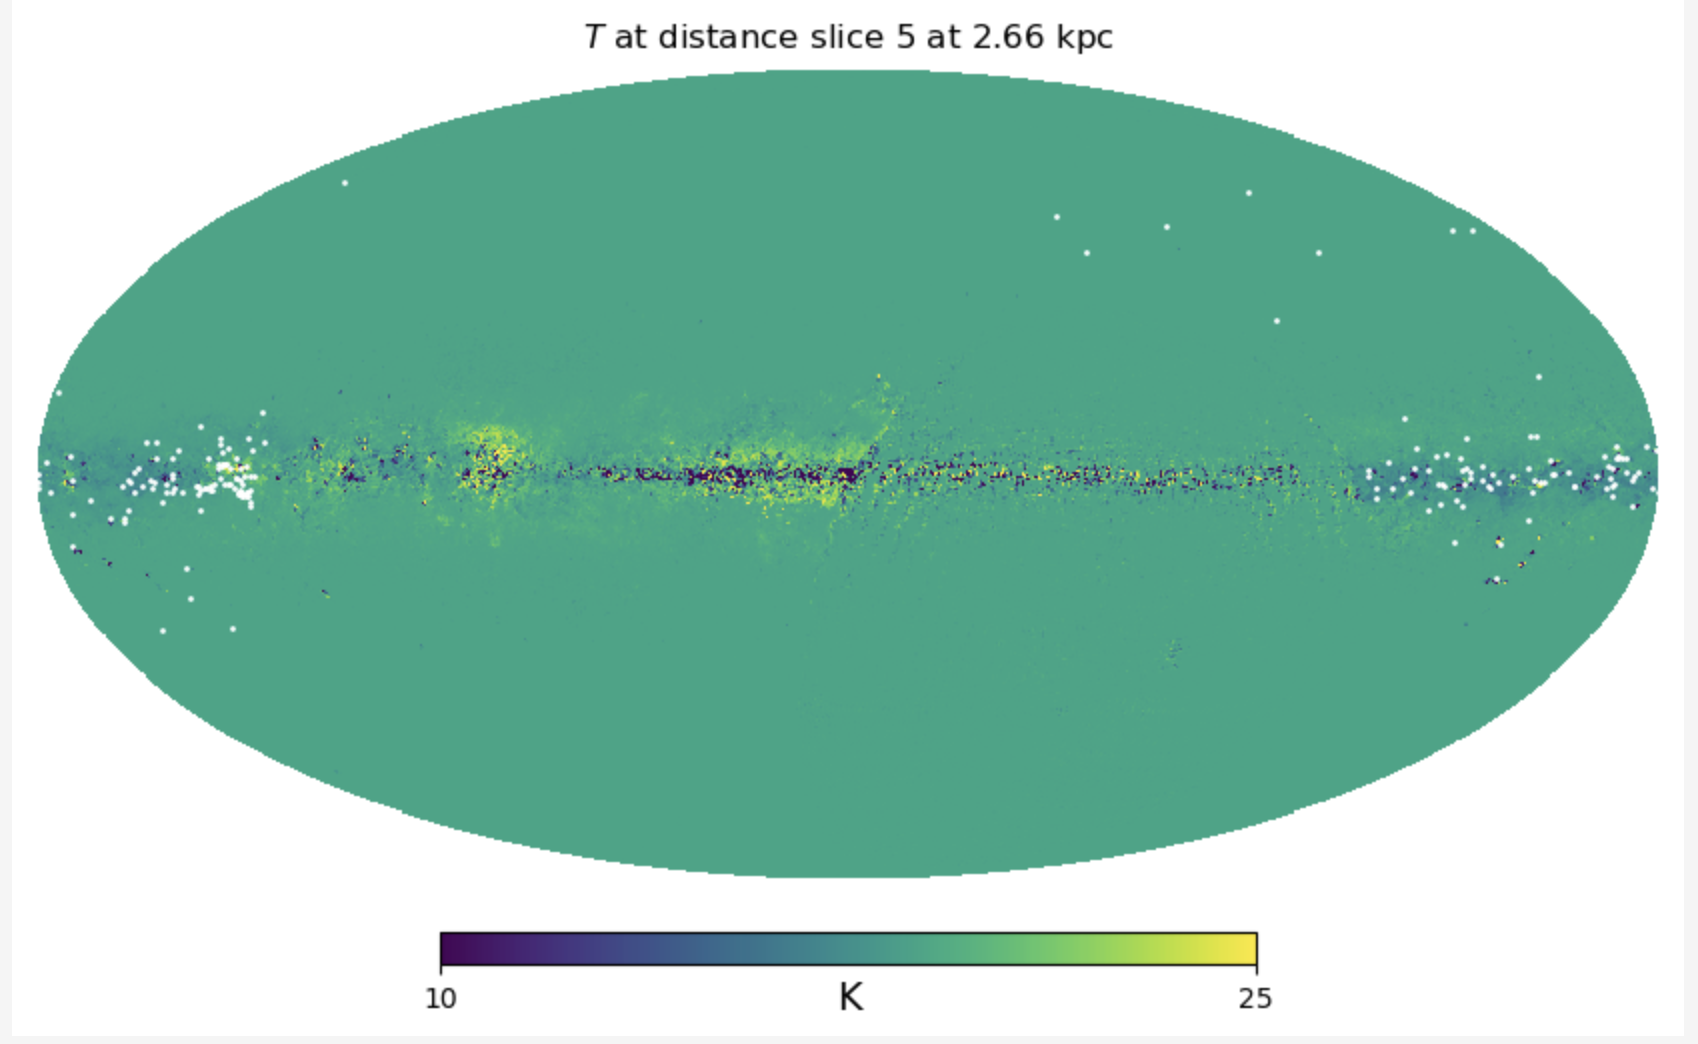
\includegraphics[scale = 0.4]{Images/Image.png}
\textbf{Figure 1:} Temperature map slice 5 with stars between 1.50kpc and 2.66kpc. White dots indicate stars taken from the big-data.csv file. The size of the stars are not to scale and were sized up for higher contrast. More figures can be generated in the code.
\end{center}


\end{document}
